% Options for packages loaded elsewhere
\PassOptionsToPackage{unicode}{hyperref}
\PassOptionsToPackage{hyphens}{url}
%
\documentclass[
]{article}
\usepackage{amsmath,amssymb}
\usepackage{iftex}
\ifPDFTeX
  \usepackage[T1]{fontenc}
  \usepackage[utf8]{inputenc}
  \usepackage{textcomp} % provide euro and other symbols
\else % if luatex or xetex
  \usepackage{unicode-math} % this also loads fontspec
  \defaultfontfeatures{Scale=MatchLowercase}
  \defaultfontfeatures[\rmfamily]{Ligatures=TeX,Scale=1}
\fi
\usepackage{lmodern}
\ifPDFTeX\else
  % xetex/luatex font selection
\fi
% Use upquote if available, for straight quotes in verbatim environments
\IfFileExists{upquote.sty}{\usepackage{upquote}}{}
\IfFileExists{microtype.sty}{% use microtype if available
  \usepackage[]{microtype}
  \UseMicrotypeSet[protrusion]{basicmath} % disable protrusion for tt fonts
}{}
\makeatletter
\@ifundefined{KOMAClassName}{% if non-KOMA class
  \IfFileExists{parskip.sty}{%
    \usepackage{parskip}
  }{% else
    \setlength{\parindent}{0pt}
    \setlength{\parskip}{6pt plus 2pt minus 1pt}}
}{% if KOMA class
  \KOMAoptions{parskip=half}}
\makeatother
\usepackage{xcolor}
\usepackage[margin=1in]{geometry}
\usepackage{longtable,booktabs,array}
\usepackage{calc} % for calculating minipage widths
% Correct order of tables after \paragraph or \subparagraph
\usepackage{etoolbox}
\makeatletter
\patchcmd\longtable{\par}{\if@noskipsec\mbox{}\fi\par}{}{}
\makeatother
% Allow footnotes in longtable head/foot
\IfFileExists{footnotehyper.sty}{\usepackage{footnotehyper}}{\usepackage{footnote}}
\makesavenoteenv{longtable}
\usepackage{graphicx}
\makeatletter
\def\maxwidth{\ifdim\Gin@nat@width>\linewidth\linewidth\else\Gin@nat@width\fi}
\def\maxheight{\ifdim\Gin@nat@height>\textheight\textheight\else\Gin@nat@height\fi}
\makeatother
% Scale images if necessary, so that they will not overflow the page
% margins by default, and it is still possible to overwrite the defaults
% using explicit options in \includegraphics[width, height, ...]{}
\setkeys{Gin}{width=\maxwidth,height=\maxheight,keepaspectratio}
% Set default figure placement to htbp
\makeatletter
\def\fps@figure{htbp}
\makeatother
\setlength{\emergencystretch}{3em} % prevent overfull lines
\providecommand{\tightlist}{%
  \setlength{\itemsep}{0pt}\setlength{\parskip}{0pt}}
\setcounter{secnumdepth}{-\maxdimen} % remove section numbering
\newlength{\cslhangindent}
\setlength{\cslhangindent}{1.5em}
\newlength{\csllabelwidth}
\setlength{\csllabelwidth}{3em}
\newlength{\cslentryspacingunit} % times entry-spacing
\setlength{\cslentryspacingunit}{\parskip}
\newenvironment{CSLReferences}[2] % #1 hanging-ident, #2 entry spacing
 {% don't indent paragraphs
  \setlength{\parindent}{0pt}
  % turn on hanging indent if param 1 is 1
  \ifodd #1
  \let\oldpar\par
  \def\par{\hangindent=\cslhangindent\oldpar}
  \fi
  % set entry spacing
  \setlength{\parskip}{#2\cslentryspacingunit}
 }%
 {}
\usepackage{calc}
\newcommand{\CSLBlock}[1]{#1\hfill\break}
\newcommand{\CSLLeftMargin}[1]{\parbox[t]{\csllabelwidth}{#1}}
\newcommand{\CSLRightInline}[1]{\parbox[t]{\linewidth - \csllabelwidth}{#1}\break}
\newcommand{\CSLIndent}[1]{\hspace{\cslhangindent}#1}
\usepackage{float}
\floatplacement{figure}{H}
\ifLuaTeX
  \usepackage{selnolig}  % disable illegal ligatures
\fi
\IfFileExists{bookmark.sty}{\usepackage{bookmark}}{\usepackage{hyperref}}
\IfFileExists{xurl.sty}{\usepackage{xurl}}{} % add URL line breaks if available
\urlstyle{same}
\hypersetup{
  pdftitle={Manuscript Demo},
  pdfauthor={Anonymous},
  hidelinks,
  pdfcreator={LaTeX via pandoc}}

\title{Manuscript Demo}
\author{Anonymous}
\date{2024-09-17}

\begin{document}
\maketitle

\hypertarget{abstract}{%
\section{Abstract}\label{abstract}}

Pretend there is an incredibly informative abstract written here.

\hypertarget{introduction}{%
\section{Introduction}\label{introduction}}

The Northern Californian ecoregion displays high numbers of documented
marine introductions, which can pose major threats to ecosystem health
and function. As of 2008, there were 85 introduced marine species
identified in Northern California, 66\% of which were considered
ecologically harmful (Molnar et al. 2008). To prevent subsequent
invasions, it is critical to fully understand which factors impact the
success of non-native species. When non-native species are first
introduced, they face a gauntlet of biotic and abiotic obstacles that
determine whether they successfully establish a population (Crowl et al.
2008). Of the abiotic factors, temperature is often considered the most
limiting (Somero 2002), particularly for organisms that are ectothermic.
Not only do invasive species typically tolerate a broad range of
temperatures, a wider geographic range is correlated with a higher upper
thermal limit, and invasive species are more likely to increase their
upper thermal limit through acclimation (Kelley 2014). While abiotic
tolerance and asexual reproduction are frequently cited as important
traits for invasion success in anemones (Gimenez and Brante 2021), the
potential for anemone-associated microbial communities to mitigate
temperature stress is largely unexplored.

Broadly, microbial communities may include both obligate and transient
members, forming a network of symbiotic relationships that can be
pathogenic, beneficial, or commensal in nature (Ayres 2016). Mutualist
community members can provide beneficial services to their host, such as
enhancing disease resistance (Lawley et al. 2012; Rosado et al. 2019),
improving nutrient acquisition (Roeselers and Newton 2012), and
facilitating environmental acclimation. For example, green frog tadpoles
that were depleted of their microbiota showed a substantial increase in
gene expression under heat stress, suggesting the tadpole microbial
community was effectively alleviating the stress response of the host
(Fontaine and Kohl 2023). Extensive research on the model anemone
\emph{Exaiptasia diaphana} has also highlighted the importance of
host-microbe interactions in host resilience during bleaching events
(Cziesielski et al. 2018). Similarly, transplanting bacteria from
heat-acclimated \emph{Nematostella vectensis} to bacteria-depleted
anemones reduces mortality at high temperatures (Baldassarre et al.
2022). Microbiota may alter host gene expression by generating molecules
that directly bind to host transcription factors (Nichols and Davenport
2020) or by producing metabolites that act as ligands for host proteins
(Chen et al. 2019). Although hosts may develop mechanisms to recruit and
maintain beneficial bacteria from the environment (Nyholm and
McFall-Ngai 2004), these mechanisms are not well understood in anemones.

Once the anemone has recruited bacteria from the environment, it is
advantageous to maintain and ``buffer'' their microbial community.
Buffering is the anemone's ability to guard their microbiota against
environmental stress, maintaining community compositions markedly
different from the surrounding water and preserving beneficial microbial
community members (Hartman, Oppen, and Blackall 2020; Muller, Fine, and
Ritchie 2016). Hartman, Oppen, and Blackall (2020) proposed that there
may be a temperature stress threshold at which significant community
changes start to occur. In a two-year experiment, Exaiptasia diaphana
reared at 32°C displayed higher richness and beta-diversity in their
microbial community than anemones reared at 25°C (Ahmed et al. 2019).
This pattern has been dubbed the `Anna Karenina Principle', where
beta-diversity is used as a proxy for host health and the stability of
the community decreases under stressed conditions (Zaneveld, McMinds,
and Vega Thurber 2017). Although prior work has largely focused on host
resilience towards warming waters, using beta-diversity to identify
microbial community stress could be further applied towards
investigating temperature tolerance in invasive species during range
expansion.

Here, I explore whether host-associated microbial communities have the
capacity to enhance invasion success by investigating the widespread
non-native anemone \emph{Diadumene lineata}'s ability to maintain a
stable microbial community at it's upper thermal limit.This work
highlights the potential for \emph{D. lineata} to be further developed
as a model organism for investigating host selection mechanisms on
microbial communities under a variety of abiotic stressors.

\hypertarget{methods}{%
\section{Methods}\label{methods}}

After collection and cleaning, anemones were fed ahead of the experiment
and recieved a fresh water change for optimal health. They were then be
placed into a beaker together for 3 days to acclimate before being
seperated for the temperature treatment (which will be for 3 more days).
Seperating the anemones is important because if any die due to heat
stress, it rapidly fouls the water. At the end of the trial, the
anemones were be macerated in DNA/RNA shield. The water was collected
and centrifuged, then the pellet was also preserved in DNA/RNA shield
until the DNA can be extracted. Each treatment had n=10 anemones,
however only 5 were selected for DNA extraction. Extra anemones were
added to account for unpredictable death that can occur when the anemone
was damaged during collection did not have time to regenerate.

\hypertarget{results}{%
\section{Results}\label{results}}

There was a significant difference in microbial community composition
between temperature treatments (PERMANOVA F = 7.8337, P = 0.001 ***).
There was still some overlap in composition between temperatures
20C-25C, with the community shifting at 27.5C and showing a substantial
difference at 30C (Figure 1). See a posthoc pairwise comparison of
treatments in Table 1.

\begin{figure}

{\centering 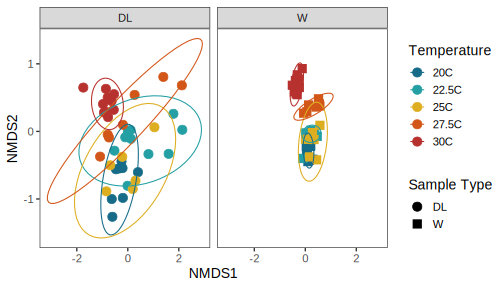
\includegraphics[width=0.8\linewidth]{../03_figs/LivingData2024_bray_NMDS} 

}

\caption{NMDS ordination of the bacterial community composition on Diadumene lineata and the surrounding water. This is a single ordination that has been faceted by sample type for visibility. Ellipses for each temperature treatment represent standard error. k = 2, stress = 0.14, using a bray-curtis dissimilarity matrix.}\label{fig:unnamed-chunk-1}
\end{figure}

\begin{longtable}[]{@{}llllll@{}}
\caption{Output of a pairwise comparison of the PERMANOVA for
temperature treatment using a bray-curtis dissimilarity matrix, 999
permuations, and the Benjamini-Hochberg p-value adjustment for multiple
comparisons.}\tabularnewline
\toprule\noalign{}
pairs & SumOfSqs & F.Model & R2 & pval & p.adj \\
\midrule\noalign{}
\endfirsthead
\toprule\noalign{}
pairs & SumOfSqs & F.Model & R2 & pval & p.adj \\
\midrule\noalign{}
\endhead
\bottomrule\noalign{}
\endlastfoot
20C vs 20CW & 0.5505471 & 6.935556 & 0.3023932 & 0.001 & 0.0014516 \\
20C vs 22.5C & 0.8376580 & 5.156749 & 0.2437401 & 0.001 & 0.0014516 \\
20C vs 22.5CW & 1.0955235 & 12.518126 & 0.4389533 & 0.001 & 0.0014516 \\
20C vs 25C & 0.3366253 & 2.175338 & 0.1534593 & 0.017 & 0.0182143 \\
20C vs 25CW & 0.7386139 & 6.757912 & 0.3602699 & 0.002 & 0.0025714 \\
20C vs 27.5C & 0.8712805 & 4.931608 & 0.2750232 & 0.001 & 0.0014516 \\
20C vs 27.5CW & 1.2041211 & 10.380849 & 0.4439894 & 0.001 & 0.0014516 \\
20C vs 30C & 1.3145343 & 10.460361 & 0.3953219 & 0.001 & 0.0014516 \\
20C vs 30CW & 1.8253622 & 21.190747 & 0.5697855 & 0.001 & 0.0014516 \\
20CW vs 22.5C & 0.7096597 & 6.037466 & 0.2511690 & 0.001 & 0.0014516 \\
20CW vs 22.5CW & 0.6912903 & 13.569781 & 0.4298345 & 0.001 &
0.0014516 \\
20CW vs 25C & 0.5526547 & 5.632375 & 0.2868922 & 0.004 & 0.0047368 \\
20CW vs 25CW & 0.4322366 & 7.305745 & 0.3429002 & 0.002 & 0.0025714 \\
20CW vs 27.5C & 0.9503507 & 7.860695 & 0.3438520 & 0.001 & 0.0014516 \\
20CW vs 27.5CW & 0.8737970 & 12.791403 & 0.4602648 & 0.001 &
0.0014516 \\
20CW vs 30C & 1.8181682 & 21.426186 & 0.5434506 & 0.001 & 0.0014516 \\
20CW vs 30CW & 1.7122971 & 34.438251 & 0.6567391 & 0.001 & 0.0014516 \\
22.5C vs 22.5CW & 0.2222768 & 1.781444 & 0.0900563 & 0.063 &
0.0630000 \\
22.5C vs 25C & 0.4596415 & 2.381002 & 0.1453514 & 0.010 & 0.0115385 \\
22.5C vs 25CW & 0.4555726 & 2.956570 & 0.1743613 & 0.003 & 0.0036486 \\
22.5C vs 27.5C & 0.4978459 & 2.376408 & 0.1367606 & 0.014 & 0.0153659 \\
22.5C vs 27.5CW & 0.6772766 & 4.316412 & 0.2234583 & 0.001 &
0.0014516 \\
22.5C vs 30C & 1.3590081 & 8.564063 & 0.3223928 & 0.001 & 0.0014516 \\
22.5C vs 30CW & 1.4760696 & 11.947065 & 0.3989394 & 0.001 & 0.0014516 \\
22.5CW vs 25C & 0.6691602 & 6.229512 & 0.3079418 & 0.001 & 0.0014516 \\
22.5CW vs 25CW & 0.4375565 & 6.391363 & 0.3134348 & 0.001 & 0.0014516 \\
22.5CW vs 27.5C & 0.7541824 & 5.820388 & 0.2795523 & 0.002 &
0.0025714 \\
22.5CW vs 27.5CW & 0.6773630 & 8.798275 & 0.3697022 & 0.001 &
0.0014516 \\
22.5CW vs 30C & 1.7158651 & 18.632876 & 0.5086381 & 0.001 & 0.0014516 \\
22.5CW vs 30CW & 1.6414270 & 28.821468 & 0.6155610 & 0.001 &
0.0014516 \\
25C vs 25CW & 0.3173596 & 2.242566 & 0.1831778 & 0.029 & 0.0303488 \\
25C vs 27.5C & 0.4865466 & 2.229676 & 0.1685360 & 0.011 & 0.0123750 \\
25C vs 27.5CW & 0.7286159 & 4.973373 & 0.3113539 & 0.001 & 0.0014516 \\
25C vs 30C & 0.9773321 & 6.471481 & 0.3161218 & 0.001 & 0.0014516 \\
25C vs 30CW & 1.2790295 & 12.083885 & 0.4632701 & 0.001 & 0.0014516 \\
25CW vs 27.5C & 0.5541842 & 3.286349 & 0.2300342 & 0.002 & 0.0025714 \\
25CW vs 27.5CW & 0.4367086 & 4.505795 & 0.2905878 & 0.003 & 0.0036486 \\
25CW vs 30C & 1.2560935 & 11.208693 & 0.4446360 & 0.001 & 0.0014516 \\
25CW vs 30CW & 1.2029665 & 17.984593 & 0.5622893 & 0.001 & 0.0014516 \\
27.5C vs 27.5CW & 0.3264860 & 1.909901 & 0.1373051 & 0.030 &
0.0306818 \\
27.5C vs 30C & 0.8416129 & 4.942736 & 0.2478464 & 0.001 & 0.0014516 \\
27.5C vs 30CW & 1.0626874 & 8.295189 & 0.3560902 & 0.001 & 0.0014516 \\
27.5CW vs 30C & 1.1676037 & 9.921442 & 0.3981087 & 0.001 & 0.0014516 \\
27.5CW vs 30CW & 0.9978611 & 13.213014 & 0.4683305 & 0.001 &
0.0014516 \\
30C vs 30CW & 0.5126671 & 5.642045 & 0.2386446 & 0.001 & 0.0014516 \\
\end{longtable}

\hypertarget{discussion}{%
\section{Discussion}\label{discussion}}

Pretend there is a detailed and nuanced discussion of the results
written up here.

\hypertarget{references}{%
\section*{References}\label{references}}
\addcontentsline{toc}{section}{References}

\hypertarget{refs}{}
\begin{CSLReferences}{1}{0}
\leavevmode\vadjust pre{\hypertarget{ref-ahmed_long-term_2019}{}}%
Ahmed, Hanin Ibrahim, Marcela Herrera, Yi Jin Liew, and Manuel Aranda.
2019. {``Long-Term Temperature Stress in the Coral Model Aiptasia
Supports the {`Anna Karenina Principle'} for Bacterial Microbiomes.''}
\emph{Frontiers in Microbiology} 10: 975.
doi:\href{https://doi.org/10.3389/fmicb.2019.00975}{10.3389/fmicb.2019.00975}.

\leavevmode\vadjust pre{\hypertarget{ref-ayres_cooperative_2016}{}}%
Ayres, Janelle S. 2016. {``Cooperative Microbial Tolerance Behaviors in
Host-Microbiota Mutualism.''} \emph{Cell} 165 (6): 1323--31.
doi:\href{https://doi.org/10.1016/j.cell.2016.05.049}{10.1016/j.cell.2016.05.049}.

\leavevmode\vadjust pre{\hypertarget{ref-baldassarre_microbiota_2022}{}}%
Baldassarre, Laura, Hua Ying, Adam M. Reitzel, Sören Franzenburg, and
Sebastian Fraune. 2022. {``Microbiota Mediated Plasticity Promotes
Thermal Adaptation in the Sea Anemone Nematostella Vectensis.''}
\emph{Nature Communications} 13 (1): 3804.
doi:\href{https://doi.org/10.1038/s41467-022-31350-z}{10.1038/s41467-022-31350-z}.

\leavevmode\vadjust pre{\hypertarget{ref-chen_forward_2019}{}}%
Chen, Haiwei, Phu-Khat Nwe, Yi Yang, Connor E. Rosen, Agata A. Bielecka,
Manik Kuchroo, Gary W. Cline, et al. 2019. {``A Forward Chemical Genetic
Screen Reveals Gut Microbiota Metabolites That Modulate Host
Physiology.''} \emph{Cell} 177 (5): 1217--1231.e18.
doi:\href{https://doi.org/10.1016/j.cell.2019.03.036}{10.1016/j.cell.2019.03.036}.

\leavevmode\vadjust pre{\hypertarget{ref-crowl_spread_2008}{}}%
Crowl, Todd A., Thomas O. Crist, Robert R. Parmenter, Gary Belovsky, and
Ariel E. Lugo. 2008. {``The Spread of Invasive Species and Infectious
Disease as Drivers of Ecosystem Change.''} \emph{Front Ecol Environ ;
6(5):238--246,}.
\url{https://www.fs.usda.gov/research/treesearch/30002}.

\leavevmode\vadjust pre{\hypertarget{ref-cziesielski_multi-omics_2018}{}}%
Cziesielski, Maha J., Yi Jin Liew, Guoxin Cui, Sebastian Schmidt-Roach,
Sara Campana, Claudius Marondedze, and Manuel Aranda. 2018.
{``Multi-Omics Analysis of Thermal Stress Response in a Zooxanthellate
Cnidarian Reveals the Importance of Associating with Thermotolerant
Symbionts.''} \emph{Proceedings of the Royal Society B: Biological
Sciences} 285 (1877).
doi:\href{https://doi.org/10.1098/rspb.2017.2654}{10.1098/rspb.2017.2654}.

\leavevmode\vadjust pre{\hypertarget{ref-fontaine_microbiome_2023}{}}%
Fontaine, Samantha S., and Kevin D. Kohl. 2023. {``The Microbiome
Buffers Tadpole Hosts from Heat Stress: A Hologenomic Approach to
Understand Host--Microbe Interactions Under Warming.''} \emph{Journal of
Experimental Biology} 226 (1): jeb245191.
doi:\href{https://doi.org/10.1242/jeb.245191}{10.1242/jeb.245191}.

\leavevmode\vadjust pre{\hypertarget{ref-gimenez_non-native_2021}{}}%
Gimenez, Lucas, and Antonio Brante. 2021. {``Do Non-Native Sea Anemones
(Cnidaria: Actiniaria) Share a Common Invasion Pattern? -- a Systematic
Review.''} \emph{Aquatic Invasions} 16 (3): 365--90.
doi:\href{https://doi.org/10.3391/ai.2021.16.3.01}{10.3391/ai.2021.16.3.01}.

\leavevmode\vadjust pre{\hypertarget{ref-hartman_effect_2020}{}}%
Hartman, Leon M., Madeleine J. H. van Oppen, and Linda L. Blackall.
2020. {``The Effect of Thermal Stress on the Bacterial Microbiome of
Exaiptasia Diaphana.''} \emph{Microorganisms} 8 (1): 20.
doi:\href{https://doi.org/10.3390/microorganisms8010020}{10.3390/microorganisms8010020}.

\leavevmode\vadjust pre{\hypertarget{ref-kelley_role_2014}{}}%
Kelley, Amanda L. 2014. {``The Role Thermal Physiology Plays in Species
Invasion.''} \emph{Conservation Physiology} 2 (1): cou045.
doi:\href{https://doi.org/10.1093/conphys/cou045}{10.1093/conphys/cou045}.

\leavevmode\vadjust pre{\hypertarget{ref-lawley_targeted_2012}{}}%
Lawley, Trevor D., Simon Clare, Alan W. Walker, Mark D. Stares, Thomas
R. Connor, Claire Raisen, David Goulding, et al. 2012. {``Targeted
Restoration of the Intestinal Microbiota with a Simple, Defined
Bacteriotherapy Resolves Relapsing Clostridium Difficile Disease in
Mice.''} \emph{{PLoS} Pathogens} 8 (10): e1002995.
doi:\href{https://doi.org/10.1371/journal.ppat.1002995}{10.1371/journal.ppat.1002995}.

\leavevmode\vadjust pre{\hypertarget{ref-molnar_assessing_2008}{}}%
Molnar, Jennifer L., Rebecca L. Gamboa, Carmen Revenga, and Mark D.
Spalding. 2008. {``Assessing the Global Threat of Invasive Species to
Marine Biodiversity.''} \emph{Frontiers in Ecology and the Environment}
6 (9): 485--92. \url{http://www.jstor.org/stable/20440991}.

\leavevmode\vadjust pre{\hypertarget{ref-muller_stable_2016}{}}%
Muller, Erinn M., Maoz Fine, and Kim B. Ritchie. 2016. {``The Stable
Microbiome of Inter and Sub-Tidal Anemone Species Under Increasing p
{CO} 2.''} \emph{Scientific Reports} 6 (1): 37387.
doi:\href{https://doi.org/10.1038/srep37387}{10.1038/srep37387}.

\leavevmode\vadjust pre{\hypertarget{ref-nichols_relationship_2020}{}}%
Nichols, Robert G., and Emily R. Davenport. 2020. {``The Relationship
Between the Gut Microbiome and Host Gene Expression: A Review.''}
\emph{Human Genetics}, November.
doi:\href{https://doi.org/10.1007/s00439-020-02237-0}{10.1007/s00439-020-02237-0}.

\leavevmode\vadjust pre{\hypertarget{ref-nyholm_winnowing_2004}{}}%
Nyholm, Spencer V., and Margaret McFall-Ngai. 2004. {``The Winnowing:
Establishing the Squid--Vibrio Symbiosis.''} \emph{Nature Reviews
Microbiology} 2 (8): 632--42.
doi:\href{https://doi.org/10.1038/nrmicro957}{10.1038/nrmicro957}.

\leavevmode\vadjust pre{\hypertarget{ref-roeselers_evolutionary_2012}{}}%
Roeselers, Guus, and Irene L. G. Newton. 2012. {``On the Evolutionary
Ecology of Symbioses Between Chemosynthetic Bacteria and Bivalves.''}
\emph{Applied Microbiology and Biotechnology} 94 (1): 1--10.
doi:\href{https://doi.org/10.1007/s00253-011-3819-9}{10.1007/s00253-011-3819-9}.

\leavevmode\vadjust pre{\hypertarget{ref-rosado_marine_2019}{}}%
Rosado, Phillipe M., Deborah C. A. Leite, Gustavo A. S. Duarte, Ricardo
M. Chaloub, Guillaume Jospin, Ulisses Nunes da Rocha, João P. Saraiva,
et al. 2019. {``Marine Probiotics: Increasing Coral Resistance to
Bleaching Through Microbiome Manipulation.''} \emph{The {ISME} Journal}
13 (4): 921--36.
doi:\href{https://doi.org/10.1038/s41396-018-0323-6}{10.1038/s41396-018-0323-6}.

\leavevmode\vadjust pre{\hypertarget{ref-somero_thermal_2002}{}}%
Somero, George N. 2002. {``Thermal Physiology and Vertical Zonation of
Intertidal Animals: Optima, Limits, and Costs of Living1.''}
\emph{Integrative and Comparative Biology} 42 (4): 780--89.
doi:\href{https://doi.org/10.1093/icb/42.4.780}{10.1093/icb/42.4.780}.

\leavevmode\vadjust pre{\hypertarget{ref-zaneveld_stress_2017}{}}%
Zaneveld, Jesse R., Ryan McMinds, and Rebecca Vega Thurber. 2017.
{``Stress and Stability: Applying the Anna Karenina Principle to Animal
Microbiomes.''} \emph{Nature Microbiology} 2 (9): 1--8.
doi:\href{https://doi.org/10.1038/nmicrobiol.2017.121}{10.1038/nmicrobiol.2017.121}.

\end{CSLReferences}

\end{document}
